\documentclass[text.tex]{subfiles}

\begin{document}
\section{Estimate of covering radius}
To catalog all different tiles that appear in a quasicrystal for a single window, all possible local configurations of the points of the quasicrystal need to be generated. 

That is achieved by generating the language of the quasicrystal $\mathcal{L}_n$ of a sufficient length that the finite sections corresponding to the words from the language $\mathcal{L}_n$ cover the disk of the radius $2R_c$ (in more detail in the next section), where $R_c$ is the covering radius of the quasicrystal (Definition \ref{def:Delone} and Theorem \ref{the:radiusLimit}).

Since the precise value of $R_c$ is difficult to evaluate, an upper bound estimate is used instead. As a reminder, here is the definition of the covering radius $R_c$, as is in Definition \ref{def:Delone}.
$$R_c = \inf\{R>0\,|\, z\in\mathbb{R}^n \exists x\in P: \|z-x\|\leq R\}$$

The estimate is derived from an artificial quasicrystal with only the largest distances between points (largest for the given window). Such quasicrystal has, for given window, certainly larger covering radius than any other. Since all such artificial quasicrystals are different only in scale and translation, the estimate is derived form a "normalized" one (a point in the origin and a unitized distance between points).

The estimate is then evaluated as the radius of a circumscribed circle or the circumradius $R$ of a triangle with vertices $(0,0)$, $(-1,0)$ and $\left(\frac{2-\beta}{2},\frac{1}{2}\right)$, as in Figure \ref{fig:coveringRadius}. 

$$R_c \leq R = \frac{a}{2sin(\alpha)} = \frac{1}{2\left(\frac{1+\sqrt{3}}{2\sqrt{2}}\right)} = \frac{\sqrt{2}(\sqrt{3}-1)}{2}$$

\begin{figure}[h]
\centering
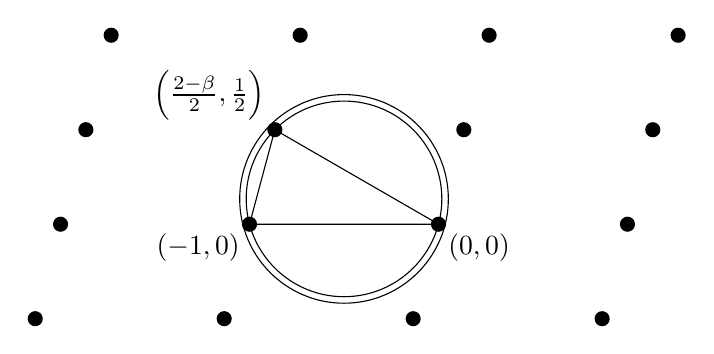
\begin{tikzpicture}[scale=2.4]

% nodes
\draw [-] (0,0)  -- (-1,0) -- (-0.86602540378,0.5) -- cycle;
\fill (1,0) circle (0.04);
\fill (0,0) circle (0.04);
\fill (-1,0) circle (0.04);
\fill (-0.86602540378,0.5) circle (0.04);
\fill (-2,0) circle (0.04);
\fill (-1.86602540378,0.5) circle (0.04);

\fill (1-0.86602540378,0.5) circle (0.04);
\fill (2-0.86602540378,0.5) circle (0.04);

\fill (-1+0.86602540378,-0.5) circle (0.04);
\fill (-2+0.86602540378,-0.5) circle (0.04);
\fill (-3+0.86602540378,-0.5) circle (0.04);
\fill (0.86602540378,-0.5) circle (0.04);

\fill (-2*0.86602540378,1) circle (0.04);
\fill (1-2*0.86602540378,1) circle (0.04);
\fill (2-2*0.86602540378,1) circle (0.04);
\fill (3-2*0.86602540378,1) circle (0.04);

\draw (-0.5,0.13397) circle (0.5176);
\draw (-0.5,0.13397) circle (0.552);

\node [below right] at (0,0) {$(0,0)$};
\node [below left] at (-1,0) {$(-1,0)$};
\node [above left] at (-0.86602540378,0.5) {$\left(\frac{2-\beta}{2},\frac{1}{2}\right)$};

\end{tikzpicture}
\caption{Section of the artificial quasicrystal with the circumcircle and a circle of the estimated radius $\hat{R}_c$.}
\label{fig:coveringRadius}
\end{figure}

Because the estimate is used in comparison with coordinates of the points of the quasicrystal, it is advantageous if it is also from $\ring$. For that the estimate $1.414 \doteq \sqrt{2} <32\beta-118 \doteq 1.426$ is used.

$$\frac{\sqrt{2}(\sqrt{3}-1)}{2} < \frac{(32\beta-118)(\beta-3)}{2} = 161-43\beta = \hat{R}_c \doteq 0.522$$

Since a unitized quasicrystal was used for the estimate, the value used in computation is the largest distance for a given window times $\hat{R}_c$.

\begin{remark}
There is an easier way that removes the need for such deriving. Simply estimate the covering radius with the largest distance itself. That is at first sufficient, but computational complexity of quasicrystals with a general window forced us to use all optimizations available.
\end{remark}
\end{document}
